\subsubsection{Umgang mit gebrochenen Funktionen}

\begin{figure}[H]
    \centering
    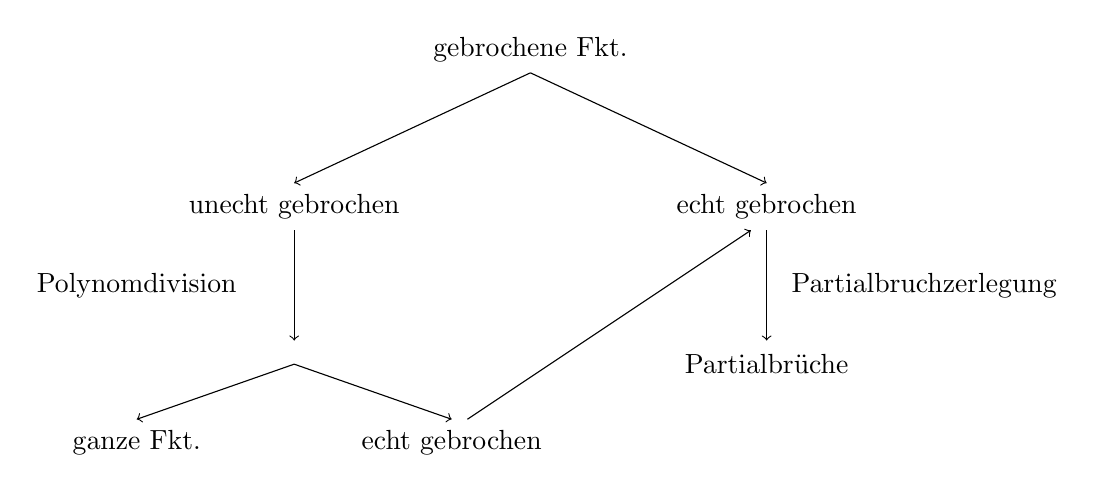
\begin{tikzpicture}
        \node[] at (0, 1) {gebrochene Fkt.};
        \node[] at (-3,-1) {unecht gebrochen};
        \node[] at (3,-1) {echt gebrochen};
        \node[] at (-5, -2) {Polynomdivision};
        \node[] at (-5, -4) {ganze Fkt.};
        \node[] at (-1, -4) {echt gebrochen};
        \node[] at (5, -2) {Partialbruchzerlegung}; 
        \node[] at (3, -3) {Partialbrüche}; 

        \draw[->] ( 0, 0.7) -- (-3,-0.7);
        \draw[->] ( 0, 0.7) -- ( 3,-0.7);
        \draw[->] (-3, -1.3) -- (-3,-2.7);
        \draw[->] (-3, -3)   -- (-5,-3.7);
        \draw[->] (-3, -3)   -- (-1,-3.7);
        
        \draw[->] (-0.8, -3.7) -- (2.8, -1.3);
        
        \draw[->] (3, -1.3) -- (3, -2.7);
    \end{tikzpicture}
    \caption{Umgang mit gebrochenen Funktionen}\label{fig:gebrochene_funktionen_graph}
\end{figure}
